% IEEE Conference Paper
% Title: Lightweight Hybrid Inertial Odometry: YOLOv26-1D with Supervised
%        Residual-Correction for Edge-Deployable Navigation
% Compiled with IEEEtran.cls (conference mode)

% \documentclass[conference]{IEEEtran}
\documentclass[10pt,conference,letterpaper]{IEEEtran}
\IEEEoverridecommandlockouts
\usepackage{cite}
\usepackage{amsmath,amssymb,amsfonts}
\usepackage{algorithmic}
\usepackage{graphicx}
\usepackage{textcomp}
\usepackage{xcolor}
% Placeholder for values not yet measured -- remove every \TBD before submission
\newcommand{\TBD}[1]{\textcolor{red}{\textbf{[#1]}}}
% Full-width (figure*) floats default to a 0.7 top-of-page fraction and a
% cramped float-page fraction, which lets a tall two-column figure (e.g.
% Fig. 2) drift several pages past the text that cites it while narrower
% single-column tables queue-jump around it. Loosen both so it settles on
% the first eligible page instead.
\renewcommand{\dbltopfraction}{0.95}
\renewcommand{\dblfloatpagefraction}{0.85}
\setcounter{dbltopnumber}{2}
% Purely typographic tightening to reclaim the last bit of page length:
% shrink table row height slightly (still comfortably legible) and trim
% the default whitespace LaTeX pads around every float, without touching
% any wording, numbers, or content.
\renewcommand{\arraystretch}{0.88}
\setlength{\textfloatsep}{6pt plus 1pt minus 1pt}
\setlength{\floatsep}{4pt plus 1pt minus 1pt}
\setlength{\intextsep}{6pt plus 1pt minus 1pt}

\def\BibTeX{{\rm B\kern-.05em{\sc i\kern-.025em b}\kern-.08em
    T\kern-.1667em\lower.7ex\hbox{E}\kern-.125emX}}

% IEEEtran lays out \and-joined authors as one continuous halign row and
% only wraps to a new row when it runs out of width, so a non-full last
% row (here: 2 authors instead of 3) inherits the same \hfill spacing
% rule as a full row: the leftover width is split evenly between the
% row's own margins AND its interior gaps, which stretches the gap
% between two authors just as much as the outer margins and leaves them
% looking like two isolated columns with an empty gap where a third
% would go. \linebreakand instead closes the current row's halign block
% and reopens a fresh one, so each row is bracketed by its own
% \hfill\mbox{}...\mbox{}\hfill and centers as an independent, tightly
% spaced unit regardless of how many authors it holds.
\makeatletter
\newcommand{\linebreakand}{%
  \end{@IEEEauthorhalign}
  \hfill\mbox{}\par
  \mbox{}\hfill\begin{@IEEEauthorhalign}
}
\makeatother

\begin{document}

% \title{Lightweight Hybrid Inertial Odometry:\\
% YOLOv26-1D with Supervised Residual-Correction\\
% for Edge-Deployable Neural Navigation}

\title{Performance-Aware Lightweight Inertial Odometry for Edge Devices via ResidualNav}

%----------Old----------
% \author{
%   \IEEEauthorblockN{Akshay Toshniwal\textsuperscript{*}}
%   \IEEEauthorblockA{\textit{Computer Science \& Engineering} \\
%   \textit{Indian Institute of Technology Kanpur}\\
%   akshayt24@iitk.ac.in}
%   \and
%   \IEEEauthorblockN{Sohel Samirkhan Modi\textsuperscript{*}}
%   \IEEEauthorblockA{\textit{Computer Science \& Engineering} \\
%   \textit{Indian Institute of Technology Kanpur} \\
%   sohelsm24@iitk.ac.in}
%   \and
%   \IEEEauthorblockN{Priyanka Bagade}
%   \IEEEauthorblockA{\textit{Computer Science \& Engineering} \\
%   \textit{Indian Institute of Technology Kanpur}\\
%   pbagade@iitk.ac.in}
% }

% Author block commented out (e.g. for double-blind review submission).
% Restore by uncommenting these lines and deleting the empty \author{} below.
% \author{
% \IEEEauthorblockN{Choudam Jaitej}
% \IEEEauthorblockA{\textit{Dept. of Comp. Sci. and Engg.} \\
% \textit{IIT Kanpur}\\
% Kanpur, India \\
% jaitejc25@iitk.ac.in}
% \and
% \IEEEauthorblockN{Akshay Toshniwal}
% \IEEEauthorblockA{\textit{Dept. of Comp. Sci. and Engg.} \\
% \textit{IIT Kanpur}\\
% Kanpur, India \\
% akshayt24@iitk.ac.in}
% \and
% \IEEEauthorblockN{Sohel Samirkhan Modi}
% \IEEEauthorblockA{\textit{Dept. of Comp. Sci. and Engg.} \\
% \textit{IIT Kanpur}\\
% Kanpur, India \\
% sohelsm24@iitk.ac.in}
% \linebreakand
% \IEEEauthorblockN{Gargi Joshi}
% \IEEEauthorblockA{\textit{Dept. of Instruments and Control Engineering} \\
% \textit{Cummins College of Engineering, Pune}\\
% Pune, India \\
% gargi.y.joshi@cumminscollege.in}
% \and
% \IEEEauthorblockN{Priyanka Bagade}
% \IEEEauthorblockA{\textit{Dept. of Comp. Sci. and Engg.} \\
% \textit{IIT Kanpur}\\
% Kanpur, India \\
% pbagade@iitk.ac.in}
% }
\author{}

\maketitle

% ============================================================
%  ABSTRACT
% ============================================================
\begin{abstract}
Deep inertial odometry can estimate pedestrian trajectories from commodity IMU streams, but accurate models remain expensive for edge devices because they require millions of parameters and their per-window velocity predictions can accumulate into long-horizon drift. This paper studies inertial odometry as a systems performance problem and quantifies the tradeoff between trajectory quality, model footprint, and inference cost under a fixed edge update budget. We propose a two-stage pipeline that combines YOLOv26-1D-Eff, a lightweight 1D convolutional backbone, with a supervised residual-correction module, \textit{ResidualNav}. The backbone regresses planar velocity from 200~Hz IMU windows using 0.60M parameters, an 87.1\% reduction relative to the 4.63M-parameter RoNIN-ResNet baseline, whereas \textit{ResidualNav} predicts local velocity errors from compact kinematic and inertial features before trajectory integration. Trained from scratch on the same public RoNIN subset and evaluated on both seen and unseen subjects, the resulting hybrid model matches the RoNIN-ResNet baseline in both Absolute and Relative Trajectory Error on seen subjects with $7.7\times$ fewer neural parameters, while trailing it on unseen subjects. On a Raspberry Pi 3 B+, the backbone runs in 25.31~ms per window, within the 50~ms update budget, $3.5\times$ faster than RoNIN-ResNet and with $3.4\times$ less energy per run. These results show that edge inertial odometry benefits from pairing a compact predictor with a low-cost correction stage to improve the accuracy--latency--footprint balance needed for real-time deployment.



\end{abstract}

\begin{IEEEkeywords}
Inertial navigation, IMU odometry, edge inference,
lightweight neural networks, residual correction, Random Forest, ATE, RTE.
\end{IEEEkeywords}

% ============================================================
%  I. INTRODUCTION
% ============================================================
\section{Introduction}

Inertial navigation estimates a user's motion from IMU measurements
alone, making it attractive for smartphones, wearables and other edge
devices that must operate without GPS or cameras \cite{ronin2019}.
Classical physics-based methods recover position by double-integrating
linear acceleration \cite{woodman2007,titterton2004}, but uncorrected
sensor biases cause position errors to diverge rapidly
\cite{woodman2007}, making pure double integration impractical without
external constraints such as zero-velocity updates \cite{foxlin2005}
or step counting \cite{jimenez2009}; these constraints often assume
specific phone placements or motion styles and can fail during
unconstrained pedestrian motion \cite{ridi2018}.

Data-driven inertial odometry relaxes some of these assumptions by
learning a direct mapping from IMU windows to velocity. RIDI
\cite{ridi2018} showed that regression-based models can estimate
velocity from inertial streams, IONet \cite{ionet2018} introduced
recurrent networks, and RoNIN \cite{ronin2019} established a benchmark
with 100 subjects and several neural backbones, including ResNet-18
\cite{resnet2016}, LSTM \cite{lstm1997} and TCN \cite{tcn2018}.
RoNIN-ResNet is a strong accuracy baseline among these, but its 4.63M
parameters and independent window-by-window predictions raise two
deployment concerns: memory/compute cost on edge processors and
short-range velocity jitter that accumulates into trajectory drift.
This makes inertial odometry a systems performance problem in which
trajectory quality, latency, and model footprint must be evaluated
together.

This paper studies that tradeoff: how much model footprint and
inference cost can be reduced while preserving trajectory quality
under a real-time IMU budget. Our approach splits the task into two
stages: a compact predictor estimates motion, and ResidualNav
learns recurring residual errors before velocity is integrated into
position. The goal is to identify a more favorable operating point
for edge navigation rather than simply optimizing accuracy in
isolation. The main contributions are:
\begin{itemize}
  \item We frame edge inertial odometry as a systems tradeoff problem and quantify the balance among trajectory quality, model footprint, and inference cost under a fixed IMU update budget.
  \item We design YOLOv26-1D-Eff, a lightweight YOLOv26-inspired 1D convolutional backbone for IMU-to-velocity regression whose attention and fusion modules are sized to the short token sequence it processes, reducing the neural parameter count from 4.63M to 0.60M while retaining competitive trajectory accuracy after correction.
  \item We introduce \textit{ResidualNav}, a supervised residual-correction layer implemented as a multi-output Random Forest regressor that reduces short-horizon velocity error before trajectory integration.
  \item We evaluate the end-to-end pipeline using trajectory accuracy, model footprint, output rate, and inference latency to characterize edge deployability.
  \item We profile the latency, power and energy of multiple lightweight backbones on a Raspberry Pi and show that the same residual-correction idea transfers across models, indicating that the approach generalizes beyond a single architecture.
\end{itemize}

% The rest of the paper is organized as follows. Section~\ref{sec:rw}
% surveys data-driven inertial odometry and lightweight edge inference.
% Section~\ref{sec:sysmodel} defines the deployment model and objectives.
% Section~\ref{sec:method} describes the proposed methodology.
% Section~\ref{sec:exp} details the experimental setup. Section~\ref{sec:results}
% presents and discusses the results and Section~\ref{sec:conclusion}
% concludes the paper.

% ============================================================
%  II. RELATED WORK
% ============================================================
\section{Related Work}
\label{sec:rw}
Prior work on inertial odometry can be grouped into three broad lines of research: (i) learned IMU-to-velocity regression, (ii) drift correction through filtering or residual postprocessing, and (iii) efficient neural designs for edge devices. Our work builds on all three by combining a lightweight predictor with residual correction to improve the deployment tradeoff.

\subsection{Data-Driven Inertial Odometry}

Data-driven inertial odometry replaces hand-crafted motion heuristics
with learned mappings from IMU streams to velocity: RIDI
\cite{ridi2018} used Support Vector Regression to estimate velocity
from stabilized IMU data, including motions that break step-counting
methods; IONet \cite{ionet2018} extended this with recurrent models;
and RoNIN \cite{ronin2019} established a large-scale benchmark with
several neural backbones, including ResNet-18, LSTM, and TCN. Later
methods tightened the coupling between learned motion and filtering
(TLIO \cite{tlio2020}), introduced attention-based backbones (CTIN
\cite{ctin2022}), and incorporated learned uncertainty propagation
into IMU preintegration for tighter sensor-fusion coupling (AirIMU
\cite{airimu2023}). These methods improved accuracy but also
highlighted a practical deployment issue: better performance often
comes with larger models and higher inference cost.

\subsection{Postprocessing and Drift Correction in INS}
Several strategies reduce the drift that inevitably builds up in
trajectory estimates. Classical filter-based corrections, such as the
extended Kalman filter, rely on linearized motion models that break
down under aggressive or unconstrained motion \cite{kalman1960}, while
hybrid approaches combining neural predictions with optimization-based
trajectory smoothing can improve consistency \cite{ronin2019} at the
cost of added system complexity. Residual correction offers a simpler
alternative, learning structured errors left by a primary predictor,
which is the idea behind our lightweight Random Forest postprocessor
for short-horizon velocity error before trajectory integration
\cite{solin2018,breiman2001,rf_imu_2023}.


\subsection{Lightweight Neural Architectures for Edge Deployment}

Running deep neural networks on edge devices requires either post-hoc
compression or efficient-by-design architectures. Knowledge
distillation, pruning and quantization are common post-training
strategies but can be sensitive to calibration data and teacher-model
quality. Architecturally efficient designs such as MobileNetV2
\cite{mobilenet2017}, ShuffleNet \cite{shufflenet2018} and the YOLO
family achieve parameter efficiency through depthwise separable
convolutions, channel shuffling, cross-stage partial connections and
compact feature pyramids; lightweight YOLO variants have also been
adapted for navigation-adjacent tasks such as real-time indoor object
detection on mobile platforms \cite{yolonav2026}. For temporal
sensing, lightweight 1D convolutional models and TCNs \cite{ronin2019}
offer efficient alternatives to heavier recurrent networks, and LLIO
\cite{llio2022} likewise pursues a lightweight learned inertial
odometer. These results support our goal of pairing a compact backbone
with residual correction for a better accuracy--latency--footprint
tradeoff in edge inertial odometry.

% ============================================================
%  III. SYSTEM MODEL AND PERFORMANCE OBJECTIVES
% ============================================================
\section{Problem Statement and System Model}
\label{sec:sysmodel}
We study edge inertial odometry as a systems problem where trajectory accuracy must be balanced against model footprint and inference cost under a fixed real-time update budget. We consider deployment on smartphones, wearables, and embedded navigation devices that continuously process IMU data under resource constraints. The device receives accelerometer and gyroscope samples at 200~Hz and must continuously produce planar velocity estimates that are integrated into the
user's trajectory. Each inference step consumes a one-second IMU window with
shape $[200 \times 6]$ and advances every ten samples, corresponding
to an update period of 50~ms. A deployable model therefore needs to
complete preprocessing, neural inference, residual correction and
trajectory integration within this update interval or with bounded
queueing delay.

Let $M$ denote model footprint, $T_{\mathrm{inf}}$ per-window inference
latency, $T_{\mathrm{upd}}$ the 50~ms update period and
$E_{\mathrm{traj}}$ a trajectory error metric such as ATE or RTE. The
deployment objective is to minimize trajectory error while satisfying
resource constraints:
\begin{equation}
\begin{aligned}
\min_{\theta,\phi} \quad & E_{\mathrm{traj}}(\theta,\phi) \\
\mathrm{s.t.} \quad & T_{\mathrm{inf}}(\theta,\phi) \leq T_{\mathrm{upd}},\\
& M(\theta,\phi) \leq M_{\max},
\end{aligned}
\label{eq:objective}
\end{equation}
where $\theta$ are the neural-backbone parameters and $\phi$ denotes the
learned residual-correction state. For the Random Forest corrector,
$\phi$ is a tree ensemble rather than a set of neural weights, so its
complexity is reported separately using tree count, depth and storage
footprint. This formulation captures the central tradeoff studied in
this paper: reducing model size and inference cost can increase local
velocity error, but a lightweight residual corrector can recover
short-horizon accuracy before velocity integration.

To address this setting, we study a two-stage design. The first stage is a compact backbone that maps IMU windows to velocity estimates with low computational cost. The second stage is a residual-correction module that learns the structured error left by the backbone and adjusts the velocity estimate before integration. This approach separates efficient inference from targeted error refinement, aiming to improve accuracy with minimal additional cost. We compare backbone--correction combinations to identify the best tradeoff among accuracy, model size, and runtime on edge devices.


% We evaluate this tradeoff using two classes of metrics. The first class
% measures navigation quality using ATE and RTE. The second class measures
% deployment cost using neural parameter count, estimated FP32 neural
% weight memory, RF corrector complexity, real-time update period and the
% latency budget implied by the IMU sampling rate. This separates
% hardware-independent footprint analysis from hardware-dependent runtime
% measurements.



\begin{figure*}[t]
\centering
\begin{minipage}[c]{0.09\textwidth}\centering
\includegraphics[width=0.8\linewidth]{walk.png}\\[2pt]
{\scriptsize\itshape Accelerometer Data, Gyroscope Data}
\end{minipage}\hfill
\begin{minipage}[c]{0.075\textwidth}\centering
{\scriptsize IMU Window $[200{\times}6]$}\\[2pt]
$\boldsymbol{\longrightarrow}$
\end{minipage}\hfill
\begin{minipage}[c]{0.15\textwidth}\centering
{\fboxrule=1pt\fcolorbox{blue!60}{blue!15}{\parbox[c][1.3cm][c]{0.92\linewidth}{\centering\scriptsize\bfseries YOLOv26-1D-Eff Backbone}}}\\[2pt]
{\scriptsize\itshape 0.60M params}
\end{minipage}\hfill
\begin{minipage}[c]{0.075\textwidth}\centering
{\scriptsize $\hat{\mathbf{v}}_t \in \mathbb{R}^2$}\\[2pt]
$\boldsymbol{\longrightarrow}$
\end{minipage}\hfill
\begin{minipage}[c]{0.15\textwidth}\centering
{\fboxrule=1pt\fcolorbox{green!60!black}{green!12}{\parbox[c][1.3cm][c]{0.92\linewidth}{\centering\scriptsize\bfseries Random Forest Corrector}}}
\end{minipage}\hfill
\begin{minipage}[c]{0.075\textwidth}\centering
{\scriptsize $\hat{\mathbf{r}}_t$ (residual)}\\[2pt]
$\boldsymbol{\longrightarrow}$
\end{minipage}\hfill
\begin{minipage}[c]{0.16\textwidth}\centering
{\fboxrule=1pt\fcolorbox{orange!70!black}{orange!10}{\parbox[c][1.3cm][c]{0.92\linewidth}{\centering\scriptsize $\tilde{\mathbf{v}}_t = \hat{\mathbf{v}}_t + \Delta\mathbf{v}_t$}}}\\[2pt]
{\scriptsize\itshape Drift-reduced}
\end{minipage}\hfill
\begin{minipage}[c]{0.065\textwidth}\centering
{\scriptsize $\tilde{\mathbf{v}}_t$}\\[2pt]
$\boldsymbol{\longrightarrow}$
\end{minipage}\hfill
\begin{minipage}[c]{0.13\textwidth}\centering
\fbox{\includegraphics[width=0.75\linewidth]{trajectory.png}}\\[2pt]
{\scriptsize\itshape Trajectory}
\end{minipage}

\vspace{5pt}

{\scriptsize\itshape Local kinematic and inertial features $\mathbf{x}_t$ built
from the same IMU window are also passed directly to the Random Forest
corrector, alongside the backbone's velocity prediction.}

\caption{Proposed hybrid inertial odometry pipeline. Raw IMU signals
(accelerometer and gyroscope) are windowed and fed into the lightweight
YOLOv26-1D-Eff backbone to produce raw planar velocity predictions
$\hat{\mathbf{v}}_t \in \mathbb{R}^2$. A supervised Random Forest
corrector predicts the residual $\hat{\mathbf{r}}_t$ using local
kinematic and inertial features, which is applied as a correction
$\tilde{\mathbf{v}}_t = \hat{\mathbf{v}}_t + \Delta\mathbf{v}_t$
before trajectory integration.}
\label{fig:pipeline}
\end{figure*}

% ============================================================
%  III. PROPOSED METHODOLOGY
% ============================================================
\section{Proposed Methodology}
\label{sec:method}

% Our system is a two-stage hybrid pipeline. Stage 1 is a
% lightweight YOLOv26-1D neural backbone that takes windowed IMU sequences
% as input and outputs planar velocity predictions. Stage 2 is a supervised
% residual-correction postprocessor that learns to predict and cancel
% the systematic short-term error in Stage 1 outputs before trajectory
% integration. Fig.~\ref{fig:pipeline} shows the end-to-end pipeline.
Figure~\ref{fig:pipeline} shows the proposed two-stage odometry pipeline. IMU measurements are first grouped into fixed-length windows and passed through a compact 1D backbone that regresses planar velocity. The resulting prediction is then refined by ResidualNav, a supervised Random Forest model that estimates the structured residual error from local kinematic and inertial context before trajectory integration.
% The purpose of this second stage is not to replace the backbone, but to recover short-horizon errors that would otherwise accumulate into long-term drift.


\subsection{Backbone Architecture: YOLOv26-1D-Eff}

YOLOv26 is a lightweight single-stage convolutional architecture that
maps its input directly to predictions without heavy multi-stage
decoding. It uses efficient CSP/C3-style blocks and compact feature
fusion, keeping computation dense but parameter-efficient
\cite{yolo26_2025}, which makes it suitable for real-time inertial
odometry under tight memory and latency constraints. We adapt it as
YOLOv26-1D-Eff: the spatial detection operations are replaced by 1D
temporal convolutions over IMU windows, the detection head is replaced
by a two-output velocity regression head, and the attention and fusion
modules are narrowed to match the short temporal sequence they process,
which the ``Eff'' designation denotes.

Concretely, for each inference window, the backbone receives an IMU
tensor of shape $[200 \times 6]$ (200 frames at 200~Hz $=$ 1 second
of gyroscope and accelerometer readings, each in the heading-agnostic
coordinate frame as defined in \cite{ronin2019}) and regresses a 2D
planar velocity vector $\hat{\mathbf{v}}_t \in \mathbb{R}^2$. At test
time, predictions are made every ten frames and integrated to build
the full trajectory. YOLOv26-1D-Eff achieves this with only 598,530
parameters, compared to 4,634,882 for the ResNet-18 1D baseline, a
$\mathbf{87.1\%}$ reduction, and requires 4.66M multiply--accumulate
operations per window, counting convolution, dense and attention
products.

The network is assembled from three primitives. A CBS unit is a
bias-free 1D convolution followed by batch normalization and a SiLU
activation. A Bottleneck1D unit contracts and restores channel width
through three CBS units with kernels of size 1, 3 and 1 at an expansion
ratio of $0.5$, and adds an identity shortcut when its input and output
widths match. A C3k2 stage optionally downsamples by stride two, splits
the signal into two half-width pointwise branches, passes one branch
through $n$ Bottleneck1D units and merges the concatenated result with
a final pointwise CBS; this cross-stage split keeps the residual path
narrow while retaining a direct route for unprocessed features.

Table~\ref{tab:yolo_arch} lists the resulting stack. A stem of a
stride-two convolution with kernel 7 followed by stride-two max pooling
reduces the 200-sample window by $4\times$, and three C3k2 stages of
widths $(64,128,256)$ with $n=(1,2,2)$ each halve the temporal length
again. The deepest stage therefore emits seven tokens of 256 channels,
one every 32 input samples, that is, one token per 160~ms of motion.

The deepest map is then refined by a lightweight attention block applied
over those seven tokens before fusion. Although stacked convolutions
already give this stage a theoretical receptive field of 275 samples,
the corresponding \emph{effective} receptive field is far narrower in
practice (90\% of gradient sensitivity concentrates within about 97
samples, averaged over 20 random initializations), so self-attention
supplies the missing long-range coupling directly instead of through a
distance-decayed stack of convolutions. Because only seven tokens are
attended, the block stays cheap: a depthwise 3-tap convolution performs
local temporal mixing, followed by a four-head self-attention on a
256-to-96-dimensional projection and a half-width feed-forward network,
each sub-block with an identity residual connection.

A lightweight neck then fuses the three stage outputs. The two
shallower maps are adaptively average-pooled to the length of the
deepest map, all three scales are projected to 96 channels by lateral
pointwise convolutions, and the 288-channel concatenation is merged by
a further C3k2 block into 192 channels, so that fine temporal detail
from the early stages survives alongside the abstract features of the
last one at a small fusion width. Global average pooling collapses the
temporal axis, a linear layer halves the fused width, and after a ReLU
and dropout a second linear layer emits the two velocity components.
Convolutional weights use Kaiming normal initialization in fan-out
mode, batch-normalization layers start at unit scale and zero offset,
and linear layers are drawn from $\mathcal{N}(0, 0.01^2)$ with zero
bias. Every operation is a 1D convolution, normalization, attention or
dense layer, so the trained graph maps directly onto standard TFLite
operators; the exported model reproduces the PyTorch outputs to within
$2\times10^{-6}$ and is used unchanged for the Raspberry Pi
measurements of Section~\ref{sec:results}.

\begin{table}[htbp]
\caption{Layer stack of YOLOv26-1D-Eff for a $6\times200$ input.}
\label{tab:yolo_arch}
\centering
\scriptsize
\begin{tabular}{|l|l|r|}
\hline
\textbf{Stage} & \textbf{Output (C$\times$T)} & \textbf{Parameters} \\
\hline
Stem: CBS($k$7,$s$2) $+$ MaxPool  & $32\times50$  & 1,408   \\
Stage 1: C3k2 ($n{=}1$, $s$2)     & $64\times25$  & 11,456  \\
Stage 2: C3k2 ($n{=}2$, $s$2)     & $128\times13$ & 52,352  \\
Stage 3: C3k2 ($n{=}2$, $s$2)     & $256\times7$  & 207,104 \\
Attention block                   & $256\times7$  & 154,464 \\
Neck (multi-scale fusion)         & $192\times7$  & 153,024 \\
GAP $+$ regression head           & $2$           & 18,722  \\
\hline
\textbf{Total}                    &               & \textbf{598,530} \\
\hline
\end{tabular}
\end{table}

\subsection{Postprocessing with ResidualNav}
The postprocessor is a supervised residual-correction layer. The
core idea is to learn a mapping between local trajectory
context and the model's short-horizon velocity error, then use that
mapping to correct future predictions before trajectory integration.

\subsubsection{Problem Setup}

At each timestep $t$, the base model predicts planar velocity
$\hat{\mathbf{v}}_t = [\hat{v}_{x,t},\,\hat{v}_{y,t}]^\top \in \mathbb{R}^2$
against the ground-truth velocity $\mathbf{v}_t = [v_{x,t},\,v_{y,t}]^\top$,
giving the residual $\mathbf{r}_t = \mathbf{v}_t - \hat{\mathbf{v}}_t$. The
postprocessor learns a function $g_\phi(\cdot)$ over a handcrafted feature
vector $\mathbf{x}_t$ built from predicted velocity behavior and
IMU-derived local context, and applies a clipped correction:
\begin{align}
  \hat{\mathbf{r}}_t &= g_\phi(\mathbf{x}_t), \\
  \Delta \mathbf{v}_t &= \mathrm{clip}\!\left(\alpha \hat{\mathbf{r}}_t,\,-c,\,+c\right), \\
  \tilde{\mathbf{v}}_t &= \hat{\mathbf{v}}_t + \Delta \mathbf{v}_t,
\end{align}
where $\alpha$ is the correction gain and $c$ is the residual clip bound,
both tuned on the validation set.

\subsubsection{Drift Reduction Rationale}

Trajectory is obtained by integrating velocity over time, so a small
per-step velocity bias $\boldsymbol{\epsilon}_t$ accumulates over the
full trajectory horizon $T$:
\begin{align}
  \hat{\mathbf{p}}_{t+1} &= \hat{\mathbf{p}}_t + \hat{\mathbf{v}}_t \Delta t, \\
  \mathbf{e}_P(T) &\approx \sum_{t=1}^{T} \boldsymbol{\epsilon}_t \Delta t.
\end{align}
Even if the instantaneous error at any single step is small, long-horizon
drift grows without bound. The postprocessor acts as a short-term local
corrector: it predicts and removes local residual patterns in
$\hat{\mathbf{v}}_t$, reducing step-wise bias and variance,
which in turn reduces the accumulated drift reflected in trajectory
error over long paths. Improving short-term velocity predictions is therefore a
principled mechanism for controlling long-term drift growth.

\subsubsection{Feature Design for Residual Learning}

For each timestep $t$, the RF model consumes a compact feature vector
$\mathbf{x}_t$ containing:

\begin{itemize}
  \item \textbf{Predicted velocity terms:} $\hat{v}_{x,t}$,
        $\hat{v}_{y,t}$, predicted speed $\|\hat{\mathbf{v}}_t\|$,
        first-differences $\Delta \hat{v}_{x,t}$,
        $\Delta \hat{v}_{y,t}$.
  \item \textbf{IMU contextual terms:} gyroscope readings
        $(\omega_x, \omega_y, \omega_z)$, accelerometer readings
        $(a_x, a_y, a_z)$ and their L2 norms
        $\|\boldsymbol{\omega}_t\|$, $\|\mathbf{a}_t\|$.
  \item \textbf{Causal short-history statistics} over a window $W$:
        \begin{align}
          \mu_t &= \frac{1}{N_t}\sum_{k=t-W+1}^{t}z_k, \\
          \sigma_t &=
          \sqrt{\max\!\left(0,\frac{1}{N_t}
          \sum_{k=t-W+1}^{t}z_k^2 - \mu_t^2\right)}
        \end{align}
        for $z_t \in \{\|\boldsymbol{\omega}_t\|,\; \|\mathbf{a}_t\|\}$,
        where $N_t = \min(t - t_0 + 1, W)$ for causal boundary handling.
\end{itemize}

These features jointly encode the instantaneous kinematic state,
local motion smoothness (via velocity finite differences) and the
local inertial regime (via IMU norms and rolling statistics), providing
the RF with sufficient structure to predict locally coherent residual
corrections.

\subsubsection{Learning Objective and Model Choice}

The corrector is a multi-output Random Forest regressor trained to
minimize $\min_\phi \sum_t \left\| \mathbf{r}_t - g_\phi(\mathbf{x}_t) \right\|_2^2$.
Random Forests \cite{breiman2001} are chosen for four complementary reasons: (i) they
handle nonlinear feature--residual relationships without requiring
careful architecture search; (ii) they are highly robust on
structured tabular data with mixed feature scales; (iii) they offer
fast deterministic inference per sample once trained; and (iv) they
natively support multi-output regression for joint $(x, y)$
velocity residual prediction.

\subsubsection{End-to-End Pipeline}

The full inference pipeline proceeds as:
\begin{enumerate}
  \item Run the YOLOv26-1D-Eff backbone to obtain $\hat{\mathbf{v}}_t$
        for all timesteps.
  \item Construct the RF training dataset from the \emph{Train} split
        only, with inputs $\mathbf{x}_t$ and labels
        $\mathbf{r}_t = \mathbf{v}_t - \hat{\mathbf{v}}_t$ computed from
        the backbone's Train-split predictions against ground truth
        (used only at train time).
  \item Fit the RF on this Train-split dataset for every
        hyperparameter combination in the grid search (Section~\ref{sec:exp}),
        and keep the combination with the lowest residual error on the
        held-out \emph{Validation} split; the kept model is never
        refit on Validation.
  \item At inference: compute $\hat{\mathbf{v}}_t$ from the base
        model, predict $\hat{\mathbf{r}}_t = g_\phi(\mathbf{x}_t)$,
        apply $\tilde{\mathbf{v}}_t = \hat{\mathbf{v}}_t + \Delta \mathbf{v}_t$
        (clipped correction), integrate $\tilde{\mathbf{v}}_t$ to
        trajectory and evaluate ATE/RTE.
\end{enumerate}

% ============================================================
%  IV. EXPERIMENTAL SETUP
% ============================================================
\section{Experimental Setup}
\label{sec:exp}

\subsection{Dataset}

All experiments use the RoNIN benchmark \cite{ronin2019}, containing
over 42.7 hours of IMU and ground-truth 3D motion data from 100
subjects across three indoor buildings, collected on three Android
smartphone models. Here, a \emph{subject} denotes one human
participant, who may contribute several of the sequences counted in
Table~\ref{tab:dataset_splits}. Ground truth comes from a body-mounted
3D tracking phone (Asus Zenfone AR) with under 0.3~m drift per 10
minutes; both IMU and pose data are recorded at 200~Hz.

Since not every RoNIN trajectory is publicly redistributed, all
models are trained and evaluated on the same publicly accessible
subset, summarized in Table~\ref{tab:dataset_splits}: 152 sequences
from 57 subjects totaling 24.87~hours, roughly 58\% of the full
release, about 1.79M input windows at stride 10. The
\emph{validation} split, held out only for early stopping and for
selecting model and postprocessor hyperparameters
(Sections~\ref{sec:method} and~\ref{sec:exp}), is not subject-disjoint
from training: like the \emph{seen} test set, most of its subjects (10
of 12) also contribute training sequences. The \emph{unseen} test
set's 15 subjects appear in no training or validation sequence; we
verified at the subject level that this split shares no subject with
the other three, so those results carry no subject-level leakage.
Training every model on this common subset removes data-access
asymmetry: the goal is a controlled comparison of lightweight
architectures under matched data and evaluation protocol, not a
reproduction of absolute state-of-the-art accuracy.

\begin{table}[htbp]
\caption{RoNIN Subset Used for All Experiments. Subject counts overlap
across splits and do not sum to the total.}
\label{tab:dataset_splits}
\centering
\scriptsize
\resizebox{\columnwidth}{!}{%
\begin{tabular}{|l|r|r|r|r|}
\hline
\textbf{Split} & \textbf{Sequences} & \textbf{Subjects} &
\textbf{Duration (h)} & \textbf{Windows} \\
\hline
Train          & 72  & 40 & 11.88 & 853,618 \\
Validation     & 16  & 12 &  2.41 & 173,378 \\
Test (seen)    & 32  & 31 &  5.23 & 376,257 \\
Test (unseen)  & 32  & 15 &  5.35 & 384,415 \\
\hline
\textbf{Total} & \textbf{152} & \textbf{57} & \textbf{24.87} &
\textbf{1,787,668} \\
\hline
\end{tabular}%
}
\end{table}

% We evaluate under a constrained-data training regime using the RoNIN
% subset available to us. Both the YOLOv26-1D model and the ResNet-18
% 1D baseline are trained from scratch on the same subset rather than
% comparing against pretrained RoNIN models trained on the full dataset.
% This ensures a strictly fair comparison and eliminates data-access
% asymmetry as a confounding variable.

\subsection{Hardware and Edge Deployment Setup}

The experiments follow a two-stage system workflow. Model training is
performed on a GPU server, while deployment latency is measured on an
actual Raspberry Pi edge device. This separates model-learning cost from
the runtime cost that matters for resource-constrained inertial
navigation.

\begin{table}[htbp]
\caption{Training and Edge-Device Hardware Configuration}
\label{tab:hardware_config}
\centering
\scriptsize
\resizebox{\columnwidth}{!}{%
\begin{tabular}{|l|l|l|}
\hline
\textbf{Role} & \textbf{Component} & \textbf{Configuration} \\
\hline
Training server & CPU & Dual Intel Xeon Gold 6226R, 2.90~GHz, 2 sockets $\times$ 32 cores \\
Training server & Memory/GPU & 376~GiB RAM, 4 NVIDIA GPUs, $\sim$48~GiB VRAM/GPU \\
\hline
Edge device & Board/CPU & Raspberry Pi 3 B+ \cite{rpi3bplus}, ARM Cortex-A53, 4 cores @ 1.4~GHz \\
Edge device & Memory/OS & 920~MiB RAM, Raspbian GNU/Linux 12, 16~GB SD card \\
\hline
\end{tabular}
}
\end{table}

For edge deployment, trained backbones are exported to TFLite
\cite{tflite} and run on the Raspberry Pi with batch size one, a
200-sample window and step size 10, profiled over 50 runs (each
processing one seen-subject sequence drawn from a pool of nine).
Board supply voltage and current are sampled before and after each
run with an Adafruit INA219 sensor wired in-line on the supply rail
and read over I2C via the CircuitPython INA219 driver; the two
readings are averaged to give board power, which is then multiplied
by the run's elapsed wall-clock time to give energy. Latency, power and energy are
averaged over the 50 runs; profiling covers the base TFLite backbones
only (the RF corrector is excluded), capturing low-power ARM latency
and energy directly rather than workstation-side timing.

\subsection{Evaluation Metrics}

Following the standard RoNIN evaluation protocol \cite{ronin2019}, we
report Absolute Trajectory Error (ATE) and Relative Trajectory Error
(RTE). For NeurIT-based reporting, we additionally include Position
Drift Error (PDE) and Absolute Yaw Error (AYE) \cite{neurit2024}. These
metrics evaluate both global trajectory accuracy and local motion
consistency.

\begin{itemize}
  \item \textbf{Absolute Trajectory Error (ATE):} the root-mean-square
        error between estimated and ground-truth trajectories over the
        whole sequence, computed in the common global frame without
        further alignment, as in RoNIN~\cite{ronin2019}, reflecting
        global path accuracy.

  \item \textbf{Relative Trajectory Error (RTE):} the root-mean-square
        error over one-minute intervals (scaled proportionally for
        sequences shorter than one minute), following
        RoNIN~\cite{ronin2019}, capturing short-term motion consistency.

  \item \textbf{Position Drift Error (PDE):} the final position drift
        relative to the total traveled path length, indicating how far
        the estimated endpoint deviates from the true one.

  \item \textbf{Absolute Yaw Error (AYE):} the root-mean-square
        difference between the estimated and ground-truth heading
        directions~\cite{neurit2024}, reflecting directional accuracy.

\end{itemize}


To characterize deployment suitability, we also report system-performance
metrics from Section~\ref{sec:sysmodel}, separate from the
trajectory-accuracy metrics above: \textbf{parameter count}, the number
of trainable neural weights, as a hardware-independent measure of model
complexity; \textbf{FP32 weight memory}, the storage needed when each
weight is kept as a 4-byte float,
$\mathrm{FP32\ size\ (MiB)} = 4 \times \#\mathrm{parameters}/1024^2$,
giving a common memory baseline before quantization or
hardware-specific compression; \textbf{model-footprint reduction}, the
percentage decrease in size relative to RoNIN-ResNet,
$(M_{\mathrm{base}}-M_{\mathrm{model}})/M_{\mathrm{base}}\times 100\%$;
the \textbf{update budget}, the time available per prediction, which at
200~Hz with stride 10 is $T_{\mathrm{upd}}=10/200=0.05~\mathrm{s}=50~\mathrm{ms}$;
and \textbf{inference latency and overhead}, the combined backbone and
RF runtime, which a real-time implementation must keep within that
budget: $T_{\mathrm{inf}} + T_{\mathrm{RF}} \leq T_{\mathrm{upd}}$.

\subsection{Baseline and Ablation Models}

Alongside the RoNIN-ResNet baseline and proposed YOLOv26-1D-Eff
pipeline, we evaluate four competing lightweight 1D backbones to test
whether residual correction remains effective across architectures:
\begin{enumerate}
  \item \textbf{RoNIN ResNet (Baseline):} ResNet-18 1D with a
        512-unit FC head, trained with the strided velocity loss.
  \item \textbf{YOLOv26-1D-Eff (No RF):} The 0.60M-parameter backbone
        of Section~\ref{sec:method}, trained identically and evaluated
        without postprocessing.
  \item \textbf{YOLOv26-1D-Eff + RF (Proposed):} YOLOv26-1D-Eff
        predictions corrected by the supervised residual RF
        postprocessor.
  \item \textbf{Competing lightweight backbones:} TinyCNN-1D,
        LightTCN-1D, ShuffleNetV2-1D and MobileNetV2-1D, trained under
        the same protocol and evaluated with and without RF correction.
        The corrector is not refitted for these backbones: the same
        Random Forest fitted to YOLOv26-1D-Eff's residuals
        (Section~\ref{sec:method}) is applied unchanged, so their
        corrected results measure how well ResidualNav transfers
        across backbones.
\end{enumerate}

\subsection{Training Details}

All networks share the same training protocol, following
RoNIN-ResNet \cite{ronin2019}: each training sample is a 200-frame
IMU window extracted every 10 frames, the batch size is 128, the
initial learning rate of $10^{-4}$ is reduced by a factor of 0.1 when
the validation loss plateaus for 10 epochs, and the
best-validation checkpoint is kept. Input and output data are
represented in the heading-agnostic coordinate frame (HACF), rotating
ground-truth trajectories randomly on the horizontal plane per step
during training for augmentation.

The optimizer and regularization are set per architecture.
YOLOv26-1D-Eff uses Adam, no weight decay and head dropout 0.5 for up
to 100 epochs. RoNIN-ResNet and the competing backbones use MuSGD, a
momentum-SGD variant with Newton--Schulz-orthogonalized updates,
momentum 0.9, weight decay $10^{-4}$ and head dropout 0.2, for up to
100 epochs (RoNIN-ResNet, ShuffleNetV2-1D, MobileNetV2-1D) or 200
(TinyCNN-1D, LightTCN-1D); every model plateaued well before its
budget. Although RoNIN trained its ResNet with Adam, our MuSGD
retrain reproduces its published unseen-subject accuracy
(5.14/4.38 versus 5.14/4.37~m), so the baseline is not disadvantaged
by the optimizer.

The Random Forest postprocessor uses 400 estimators with a maximum
tree depth of 12, minimum samples per leaf of 1 and \texttt{sqrt}
feature sampling per split, selected via grid search on the
validation set. For YOLOv26-1D-Eff, the residual correction uses
gain $\alpha = 1.25$ and clip bound $c = 0.25$, also tuned on the
validation set.
% ============================================================
%  V. RESULTS AND DISCUSSION
% ============================================================
\section{Results and Discussion}
\label{sec:results}

\subsection{Parameter Efficiency}

Table~\ref{tab:model_footprint} separates neural backbone footprint from residual-correction complexity. YOLOv26-1D-Eff contains 0.60M trainable parameters, an 87.1\% reduction relative to RoNIN-ResNet. ResidualNav employs a 400-tree Random Forest over 17 input features; as a non-neural component, its storage cost is reported separately and is not included in the neural parameter count or FP32 weight size.

\begin{table}[htbp]
\caption{Model Footprint and Parameter Summary}
\label{tab:model_footprint}
\centering
\scriptsize
\begin{tabular}{|l|c|c|}
\hline
\textbf{Model} & \textbf{Neural Params} & \textbf{FP32 Size} \\
\hline
YOLOv26-1D-Eff & 598,530 & 2.28 MiB \\
\textbf{YOLOv26-1D-Eff + RF} & \textbf{598,530} &
\textbf{2.28 MiB} \\
RoNIN ResNet & 4,634,882 & 17.68 MiB \\
\hline
\end{tabular}
\end{table}

Table~\ref{tab:model_footprint} summarizes the static model footprint. All models process the same 200~Hz IMU stream with stride 10, corresponding to a 50~ms update budget. Because the Random Forest is a tree ensemble rather than a neural network, its storage cost is reported separately from neural FP32 weight memory. Consequently, both the neural parameter count and the Raspberry Pi profiling in Table~\ref{tab:pi_tflite_latency} describe the base backbones.

\subsection{Edge Inference on Raspberry Pi}

% Table~\ref{tab:pi_tflite_latency} reports deployed Raspberry Pi latency
% for the RF-corrected backbones and RoNIN-ResNet. Among the
% accuracy-competitive models, YOLOv26-1D + RF is faster than
% MobileNetV2 + RF and RoNIN-ResNet, while the measured RF overhead is
% only about 0.125~ms/sample. This table is the main deployment evidence
% because it reports target-device latency rather than proxy workstation
% timing. For hybrid models, reported latency includes TFLite backbone inference
% followed by RF residual correction.

Table~\ref{tab:pi_tflite_latency} reports the per-window latency, average board power and measured energy per run of the TFLite backbones on the Raspberry Pi 3 B+. YOLOv26-1D-Eff runs in 25.31~ms per window, within the 50~ms update budget with 24.7~ms of headroom, and is $3.5\times$ faster than RoNIN-ResNet (89.42~ms) and $3.2\times$ faster than MobileNetV2-1D (80.08~ms), both of which exceed the budget. Average board power varies from 3.24~W (LightTCN-1D) to 4.34~W (TinyCNN-1D), only a $1.34\times$ spread against an $8.1\times$ spread in latency, so energy is governed mainly by latency rather than power: YOLOv26-1D-Eff consumes 671.78~J per run against 2269.86~J for RoNIN-ResNet, a $3.4\times$ reduction. This latency dominance produces a \emph{race-to-sleep} effect~\cite{albers2010energy}: TinyCNN-1D draws the highest average power of any model (4.34~W) yet has the lowest energy per run (359.75~J), because its 11.09~ms latency lets the board return to a lower-power idle state sooner than the lower-power but slower alternatives. Since energy is the time integral of power, finishing a window faster at a higher draw can still cost less total energy than running longer at a lower one. TinyCNN-1D and ShuffleNetV2-1D also meet the budget, while LightTCN-1D narrowly misses it at 50.11~ms; after correction, TinyCNN-1D is less accurate on both metrics and ShuffleNetV2-1D has a higher ATE (Table~\ref{tab:seen}).


\begin{table}[htbp]
\caption{Raspberry Pi 3 B+ Profiling of the Base TFLite Backbones (Mean over 50 Runs)}
\label{tab:pi_tflite_latency}
\centering
\scriptsize
\resizebox{\columnwidth}{!}{%
\begin{tabular}{|l|c|c|c|c|}
\hline
\textbf{Model} & \textbf{Neural} & \textbf{Latency} & \textbf{Power} & \textbf{Energy} \\
 & \textbf{Params} & \textbf{(ms/window)} & \textbf{(W)} & \textbf{(J/run)} \\
\hline
LightTCN-1D & 79,628 & 50.11 & 3.24 & 1208.28 \\
TinyCNN-1D & 116,146 & 11.09 & 4.34 & 359.75 \\
\textbf{YOLOv26-1D-Eff (Ours)} & \textbf{598,530} & \textbf{25.31} & \textbf{3.54} & \textbf{671.78} \\
ShuffleNetV2-1D & 854,618 & 33.36 & 3.39 & 844.22 \\
MobileNetV2-1D & 2,642,562 & 80.08 & 3.46 & 2067.97 \\
RoNIN ResNet (Baseline) & 4,634,882 & 89.42 & 3.39 & 2269.86 \\
\hline
\end{tabular}
}
\end{table}



\subsection{Seen Test Set Performance}

% Table~\ref{tab:seen} reports ATE and RTE on seen subjects, with models ordered by increasing neural parameter count. The
% competing backbones show that RF correction is not specific to
% YOLOv26-1D. For the proposed YOLOv26-1D model, RF correction improves YOLOv26-1D from ATE/RTE 3.9573/3.0700 to 3.7359/2.5979, surpassing the RoNIN-ResNet RTE.% of 2.7201~m.

Table~\ref{tab:seen} reports ATE and RTE on seen subjects, with models ordered by increasing neural parameter count. RF correction generally improves trajectory accuracy across lightweight backbones, although the gains vary by architecture. For YOLOv26-1D-Eff, RF correction reduces ATE/RTE from 4.1649/3.1488 to 3.5848/2.6081, a 17.2\% RTE reduction, and brings it level with the RoNIN-ResNet baseline (3.7114/2.7614) at $7.7\times$ fewer neural parameters. Among the backbones that meet the 50~ms budget on the Raspberry Pi (Table~\ref{tab:pi_tflite_latency}), YOLOv26-1D-Eff+RF attains the lowest ATE, while ShuffleNetV2-1D+RF attains a slightly lower RTE (2.4248 versus 2.6081~m). Fig.~\ref{fig:trajectories} shows representative predicted trajectories for four of these seen-subject sequences.

\begin{table}[htbp]
\caption{Seen Test Set Results (Public RoNIN Subset)}
\label{tab:seen}
\centering
\scriptsize
\resizebox{\columnwidth}{!}{%
\begin{tabular}{|l|c|c|c|c|}
\hline
\textbf{Model} & \textbf{ATE} & \textbf{RTE} &
\textbf{ATE (+RF)} & \textbf{RTE (+RF)} \\
\hline
LightTCN-1D & 5.6082 & 3.3909 & 5.7823 & 3.4441 \\
TinyCNN-1D & 4.7783 & 3.1978 & 4.7689 & 2.7939 \\
YOLOv26-1D-Eff (Ours) & 4.1649 & 3.1488 & \textbf{3.5848} & \textbf{2.6081} \\
ShuffleNetV2-1D & 3.9425 & 2.8061 & 3.9048 & 2.4248 \\
MobileNetV2-1D & 3.9705 & 2.7708 & 3.8009 & 2.4261 \\
RoNIN ResNet (Baseline) & 3.7114 & 2.7614 & -- & -- \\
\hline
\end{tabular}
}
\end{table}

\begin{figure*}[t]
\centering

% Single row of four panels -- far shorter vertically than a 2x2 grid.
\begin{minipage}[t]{0.235\textwidth}
  \centering
  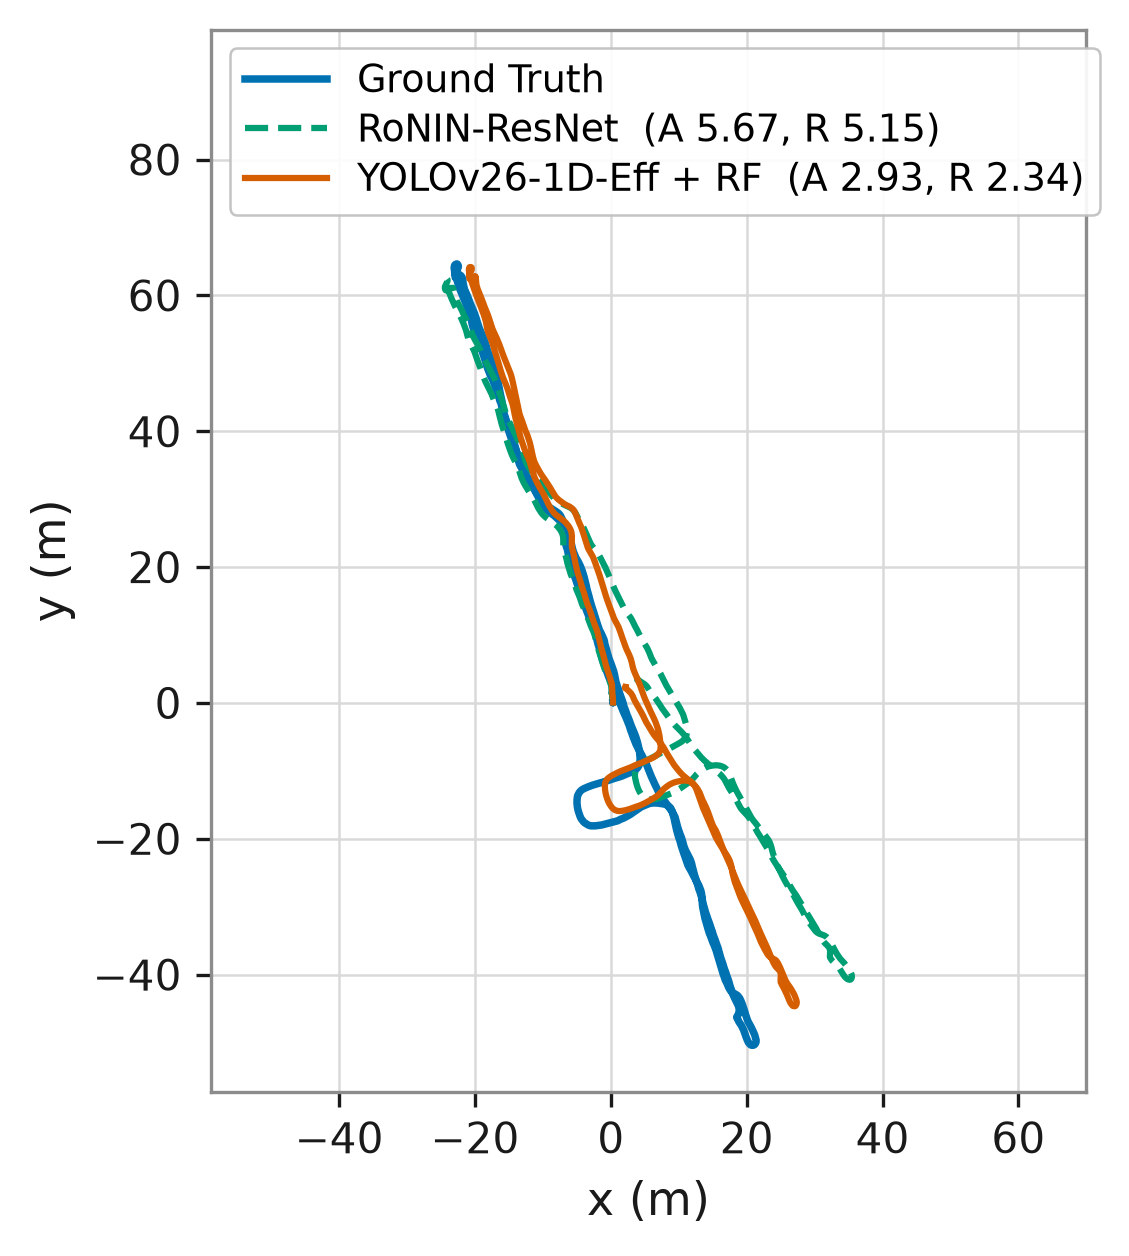
\includegraphics[width=0.98\linewidth]{traj1_large_text.png}
  \label{fig:traj1}
\end{minipage}\hfill
\begin{minipage}[t]{0.235\textwidth}
  \centering
  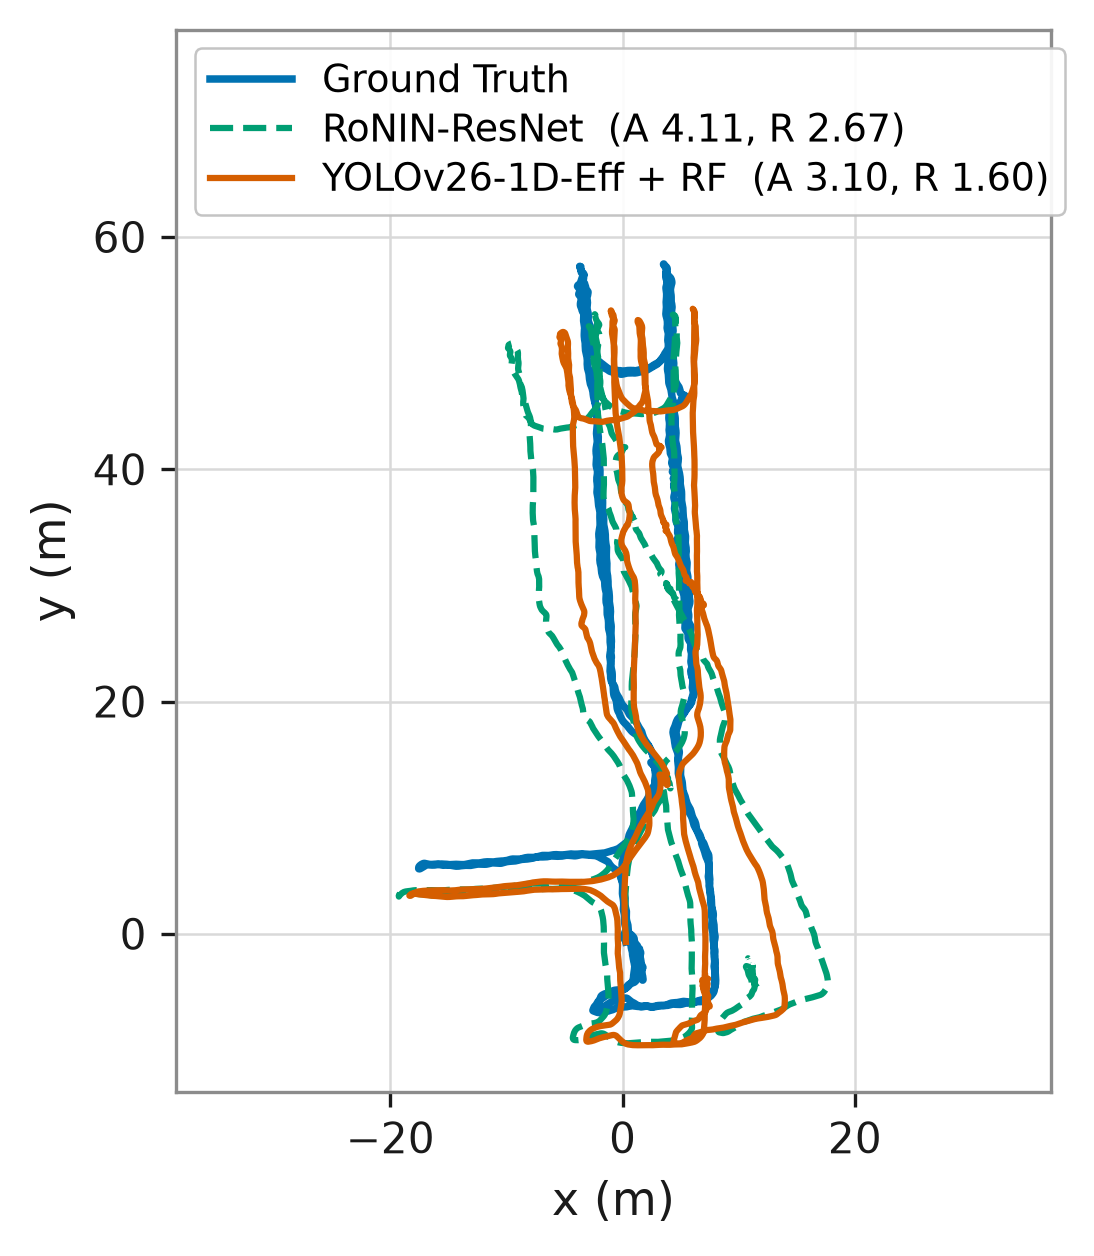
\includegraphics[width=0.98\linewidth]{traj2_large_text.png}
  \label{fig:traj2}
\end{minipage}\hfill
\begin{minipage}[t]{0.235\textwidth}
  \centering
  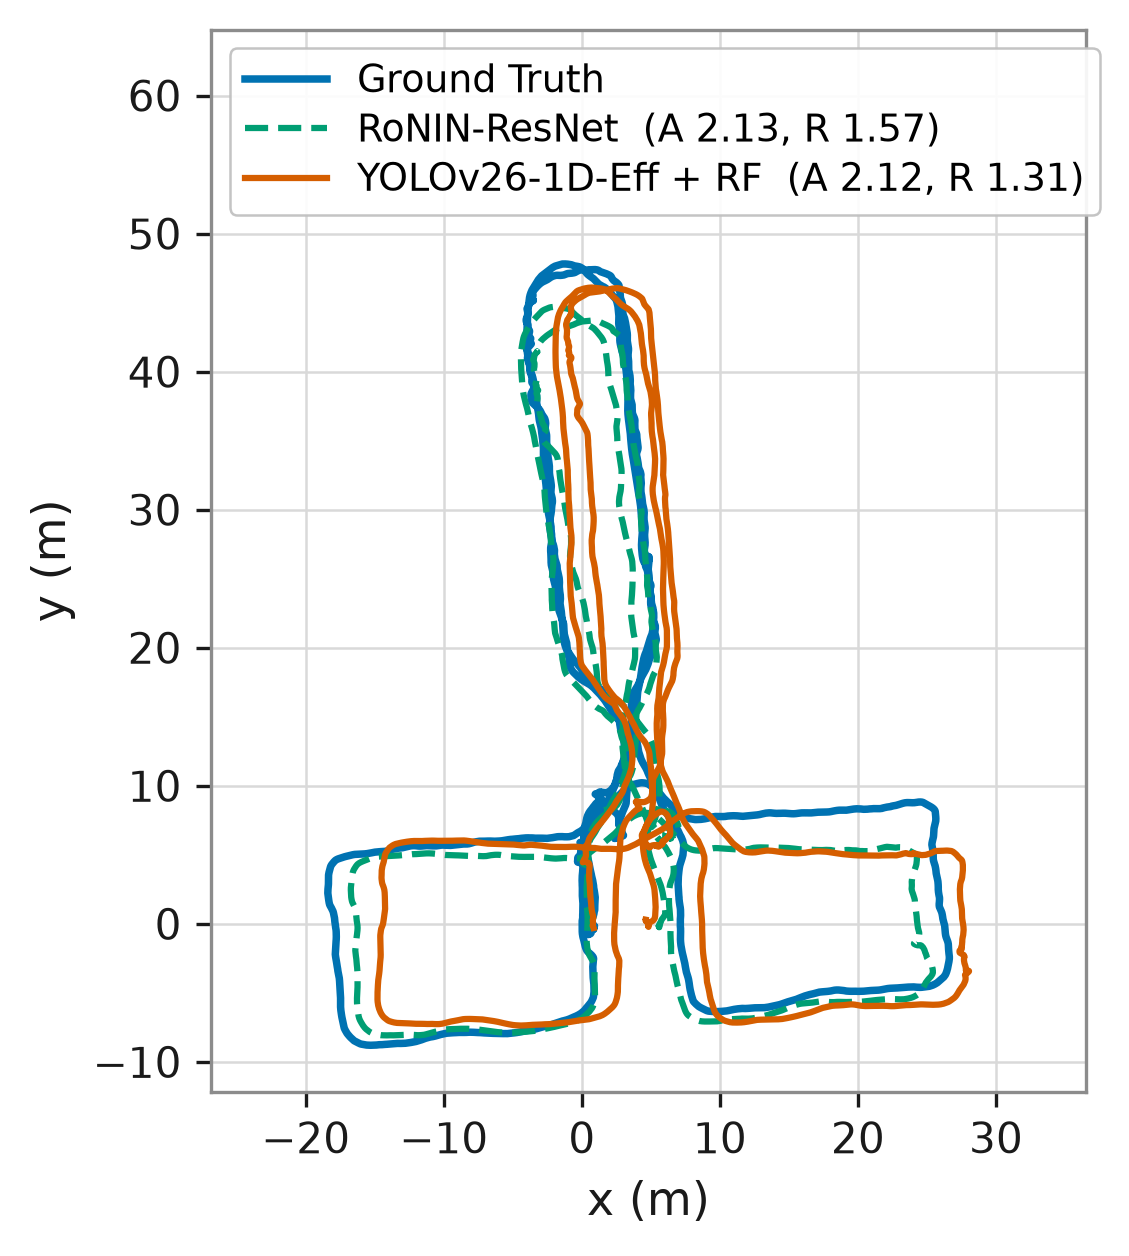
\includegraphics[width=0.98\linewidth]{traj3_large_text.png}
  \label{fig:traj3}
\end{minipage}\hfill
\begin{minipage}[t]{0.235\textwidth}
  \centering
  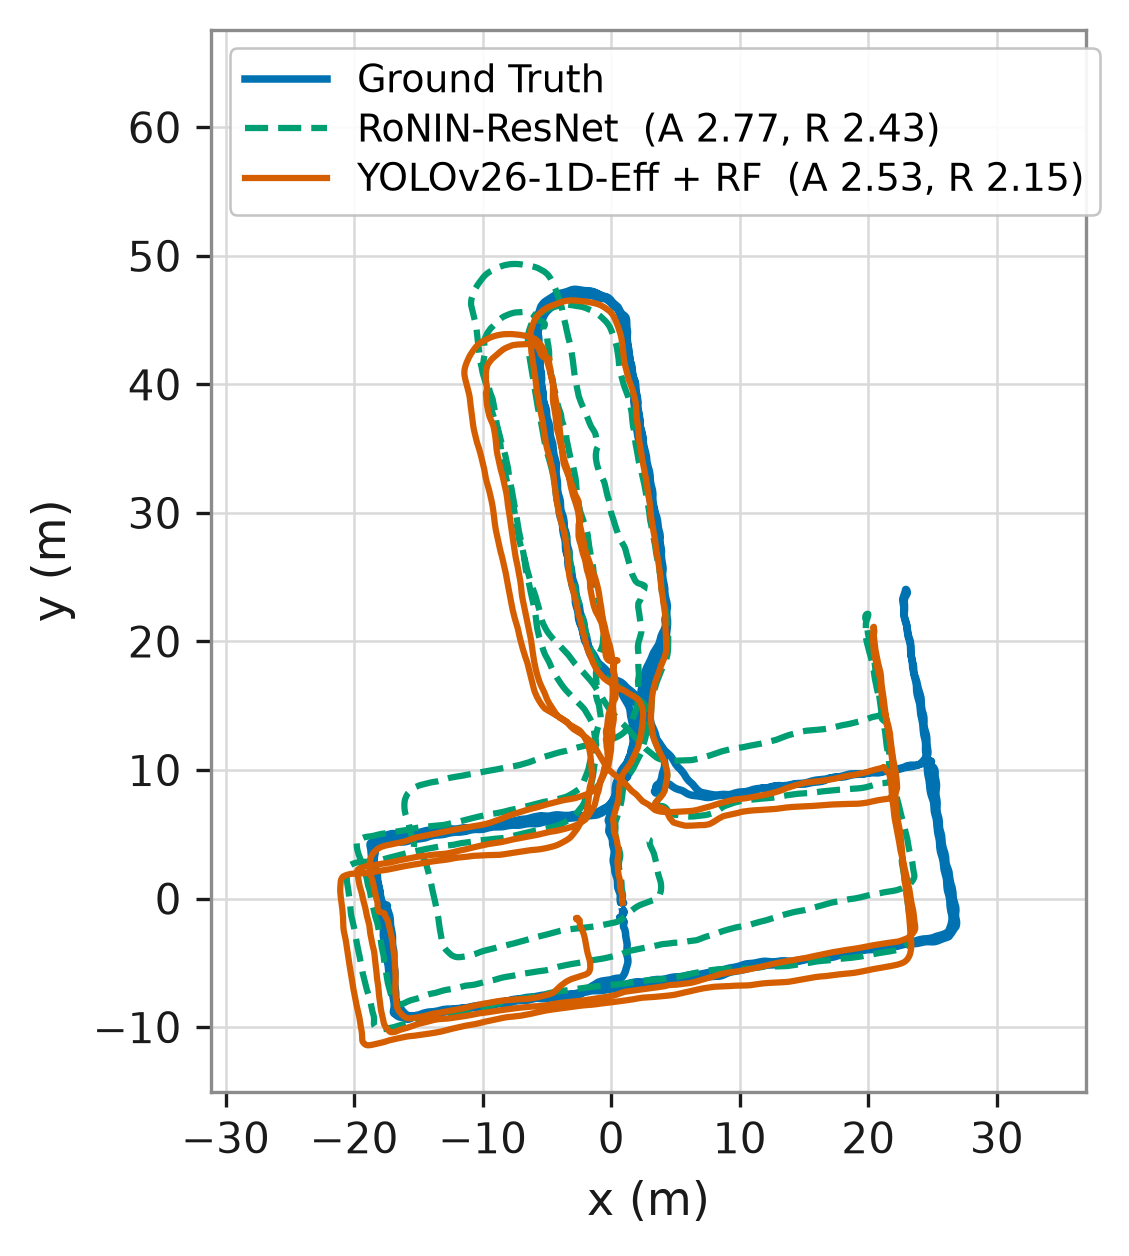
\includegraphics[width=0.98\linewidth]{traj4_large_text.png}
  \label{fig:traj4}
\end{minipage}

\caption{Trajectory comparisons between ground truth (blue, solid), the
RoNIN-ResNet baseline (green, dashed) and the proposed YOLOv26-1D-Eff + RF
hybrid (orange, solid) on four selected seen-subject sequences. On each
sequence the proposed model attains lower ATE and RTE than RoNIN-ResNet
while using $7.7\times$ fewer neural parameters; this holds for 12 of the
32 seen-subject test sequences. \textbf{``A'' denotes ATE (m) and ``R''
denotes RTE (m).}}

\label{fig:trajectories}
\end{figure*}

\subsection{Unseen Test Set Performance and Generalization}

% Table~\ref{tab:unseen} reports generalization to subjects not present in
% training. Errors
% increase for all models, but RF correction still
% improves most RTE values. YOLOv26-1D + RF reaches ATE/RTE
% 5.5368/4.2805, again improving on the RoNIN-ResNet RTE of 4.4999~m. The RoNIN-ResNet baseline retrained on the same subset achieves performance close to the original RoNIN results, supporting the validity of our comparative evaluation protocol.

Table~\ref{tab:unseen} reports generalization to unseen subjects. RF correction yields smaller gains here, reducing YOLOv26-1D-Eff RTE from 4.9368 to 4.7313 while leaving ATE essentially unchanged (5.8977 to 5.9046). The retrained RoNIN-ResNet baseline (5.1400/4.3770) is stronger on unseen subjects, so the lightweight backbones trade some cross-subject generalization for their reduced footprint. For reference, the original RoNIN study~\cite{ronin2019} reported ResNet ATE/RTE of 3.54/2.67 on seen subjects and 5.14/4.37 on unseen subjects using the full training dataset; our retrained values (3.7114/2.7614 seen, 5.1400/4.3770 unseen) are close to these published numbers, supporting the validity of the evaluation protocol despite using only the publicly accessible subset (Table~\ref{tab:dataset_splits}). MobileNetV2-1D+RF attains the lowest error among the lightweight models, but its backbone alone needs 80.08~ms per window on the Raspberry Pi, exceeding the 50~ms budget, whereas the YOLOv26-1D-Eff backbone needs 25.31~ms.

\begin{table}[htbp]
\caption{Unseen Test Set Results (Generalization)}
\label{tab:unseen}
\centering
\scriptsize
\resizebox{\columnwidth}{!}{%
\begin{tabular}{|l|c|c|c|c|}
\hline
\textbf{Model} & \textbf{ATE} & \textbf{RTE} &
\textbf{ATE (+RF)} & \textbf{RTE (+RF)} \\
\hline
LightTCN-1D & 8.6503 & 4.9925 & 8.6435 & 4.7760 \\
TinyCNN-1D & 6.5321 & 5.0162 & 6.4391 & 4.5282 \\
YOLOv26-1D-Eff (Ours) & 5.8977 & 4.9368 & \textbf{5.9046} & \textbf{4.7313} \\
ShuffleNetV2-1D & 5.7805 & 4.6046 & 5.9522 & 4.1057 \\
MobileNetV2-1D & 5.5274 & 4.5530 & 5.2699 & 4.0811 \\
RoNIN ResNet (Baseline) & 5.1400 & 4.3770 & -- & -- \\
\hline
\end{tabular}
}
\end{table}


\subsection{Analysis of Residual Correction}

% RF correction improves RTE more strongly than ATE because it operates on
% short-horizon velocity residuals before trajectory integration. This
% suggests that raw YOLOv26-1D errors contain local step-wise bias, which
% the RF can reduce using kinematic features and rolling inertial
% statistics $(\mu_t, \sigma_t)$. This also explains why the gain is
% stronger in RTE than ATE: RTE directly measures local drift, which is
% the error type targeted by ResidualNav.

RF correction consistently yields larger improvements in RTE than ATE across most backbones. Since the corrector operates on short-horizon velocity residuals prior to trajectory integration, it primarily reduces local drift rather than global trajectory error. The results suggest that lightweight backbones exhibit systematic short-term prediction errors that can be mitigated using compact kinematic features and rolling inertial statistics. Consequently, the benefits of residual correction are most evident in RTE, which directly captures local trajectory consistency.

\subsection{Stage-2 Corrector Comparison}

Table~\ref{tab:corrector_variants} compares four residual correctors on
the YOLOv26-1D-Eff backbone: (A) the Random Forest used in ResidualNav,
(B) an exponential moving average, (C) a small MLP, and (D) a temporal
convolutional network. On seen subjects the Random Forest gives the
largest reduction in both ATE (4.1649 to 3.5848) and RTE (3.1488 to
2.6081), with the MLP second. On unseen subjects the differences
between correctors are small: the MLP attains a marginally lower ATE
(5.8741 versus 5.9046), while the Random Forest attains the lowest
RTE (4.7313). The nonlinear Random Forest therefore provides the
strongest overall correction, particularly where residual structure is
shared with the training subjects, which motivates its use in
ResidualNav.

\begin{table}[htbp]
\caption{Stage-2 Residual Corrector Comparison on YOLOv26-1D-Eff (ATE / RTE, m). Best value per column in bold.}
\label{tab:corrector_variants}
\centering
\scriptsize
\resizebox{\columnwidth}{!}{%
\begin{tabular}{|l|c|c|c|c|}
\hline
\textbf{Corrector} & \textbf{Seen ATE} & \textbf{Seen RTE} &
\textbf{Unseen ATE} & \textbf{Unseen RTE} \\
\hline
None (base)      & 4.1649 & 3.1488 & 5.8977 & 4.9368 \\
A: Random Forest & \textbf{3.5848} & \textbf{2.6081} & 5.9046 & \textbf{4.7313} \\
B: EMA           & 4.1575 & 3.1220 & 5.8889 & 4.9136 \\
C: MLP           & 3.7298 & 2.8269 & \textbf{5.8741} & 4.8625 \\
D: TCN           & 4.8027 & 2.8996 & 6.7961 & 4.8896 \\
\hline
\end{tabular}%
}
\end{table}

%-------------Old
% \subsection{Cross-Model and Cross-Dataset Applicability}

% To test whether RF residual correction transfers beyond our
% YOLOv26-1D/RoNIN setup, we apply the same output-refinement stage to
% NeurIT \cite{neurit2024} and RIDI \cite{ridi2018} without changing their
% base odometry pipelines. NeurIT represents a recent neural tracker on a
% robotic multi-building dataset, while RIDI represents a classical
% smartphone inertial-odometry pipeline.

% \begin{table}[htbp]
% \caption{Residual Correction Result for NeurIT}
% \label{tab:neurit_rf_result}
% \centering
% \scriptsize
% \begin{tabular}{|l|c|c|c|c|}
% \hline
% \textbf{Configuration} & \textbf{ATE (m)} & \textbf{RTE (m)} &
% \textbf{PDE} & \textbf{AYE} \\
% \hline
% NeurIT without RF & 1.3578 & 0.6958 & 0.0105 & 38.0137 \\
% NeurIT + RF & 1.2618 & 0.6791 &
% 0.0091 & 35.6194 \\
% \hline
% \end{tabular}
% \end{table}

% Table~\ref{tab:neurit_rf_result} shows that RF improves NeurIT across
% global error, local drift, endpoint drift and yaw-direction agreement.

% \begin{figure}[H]
% \centering
% \includegraphics[width=0.9\columnwidth]{101office1.png}
% \caption{NeurIT trajectory comparison before and after RF postprocessing on
% the 101office1 sequence.}
% \label{fig:neurit_rf_comparison}
% \end{figure}

% % \begin{table}[htbp]
% % \caption{Inference-Time Summary for NeurIT Before and After RF Postprocessing}
% % \label{tab:neurit_inference_time}
% % \centering
% % \scriptsize
% % \resizebox{\columnwidth}{!}{%
% % \begin{tabular}{|l|c|c|c|}
% % \hline
% % \textbf{Configuration} & \textbf{TF-BRT/window} &
% % \textbf{Avg. time/sequence} \\
% % \hline
% % NeurIT before RF & 6.048 ms & 2.128 s  \\
% % NeurIT + RF & 6.048 ms & 2.702 s  \\
% % \hline
% % \end{tabular}
% % }
% % \end{table}

% \begin{table}[t]
% \centering
% \caption{Inference-Time Summary for NeurIT Before and After RF Postprocessing}
% \label{tab:neurit_inference_time}
% \begin{tabular}{|l|c|c|}
% \hline
% \textbf{Configuration} & \textbf{Avg. time/sequence} & \textbf{Avg. latency/sample} \\
% \hline
% NeurIT baseline        & 2.128 s & 6.048 ms \\
% NeurIT + RF            & 2.700 s & 7.676 ms \\
% RF postprocessor only  & 0.573 s & 1.628 ms \\
% \hline
% \end{tabular}
% \end{table}

% Table~\ref{tab:neurit_inference_time} shows that RF leaves the TF-BRT
% window time unchanged and adds 0.57~s over the evaluated sequence.
% RIDI provides the complementary case of human smartphone odometry with a
% placement-aware SVM/SVR pipeline.

% \begin{table}[htbp]
% \caption{Residual Correction Result for RIDI}
% \label{tab:ridi_rf_result}
% \centering
% \scriptsize
% \begin{tabular}{|l|c|c|}
% \hline
% \textbf{Configuration} & \textbf{ATE (m)} & \textbf{RTE (m)} \\
% \hline
% RIDI baseline & 2.1924 & 3.6724 \\
% RIDI + RF & 2.0892 & 3.3580 \\
% \hline
% \end{tabular}
% \end{table}

% Table~\ref{tab:ridi_rf_result} shows that RF correction also improves
% RIDI, indicating transfer to a non-neural regression-based pipeline.

% \begin{figure}[H]
% \centering
% \includegraphics[width=0.85\columnwidth]{ridi_rf_comparison_large_text.png}
% \caption{RIDI trajectory comparison before and after RF postprocessing.}
% \label{fig:ridi_rf_comparison}
% \end{figure}

% \begin{table}[htbp]
% \caption{Inference-Time Summary for RIDI Before and After RF Postprocessing}
% \label{tab:ridi_inference_time}
% \centering
% \scriptsize
% \resizebox{\columnwidth}{!}{%
% \begin{tabular}{|l|c|c|c|}
% \hline
% \textbf{Configuration} &
% \textbf{Avg. time/sequence} & \textbf{Avg. latency/sample} \\
% \hline
% RIDI baseline & 21.568 s & 1.135 ms \\
% RIDI + RF & 21.959 s & 1.158 ms \\
% RF postprocessor only & 0.390 s & 0.023 ms \\
% \hline
% \end{tabular}
% }
% \end{table}

% Table~\ref{tab:ridi_inference_time} shows that the RF-only component
% adds 0.390~s per sequence, corresponding to 0.023~ms per sample. Together, the NeurIT and RIDI results show that ResidualNav is not tied
% to one backbone, dataset, or odometry style. It can reduce predictable
% local residual structure in both neural and classical inertial-odometry
% outputs.
%----------------------

\subsection{Cross-Model and Cross-Dataset Applicability}

To evaluate portability, we apply the proposed \textit{ResidualNav} without modifying the
base pipelines of NeurIT~\cite{neurit2024}, a neural robotic tracker,
and RIDI~\cite{ridi2018}, a classical smartphone SVM/SVR pipeline.

\begin{table}[htbp]
\caption{Residual Correction Results for NeurIT and RIDI}
\label{tab:crossmodel_rf_result}
\centering
\scriptsize
\resizebox{\columnwidth}{!}{%
\begin{tabular}{|l|c|c|c|c|}
\hline
\textbf{Configuration} & \textbf{ATE (m)} & \textbf{RTE (m)} &
\textbf{PDE} & \textbf{AYE} \\
\hline
NeurIT baseline & 1.3578 & 0.6958 & 0.0105 & 38.0137 \\
NeurIT + RF & \textbf{1.2618} & \textbf{0.6791} &
\textbf{0.0091} & \textbf{35.6194} \\
\hline
RIDI baseline & 2.1924 & 3.6724 & -- & -- \\
RIDI + RF & \textbf{2.0892} & \textbf{3.3580} & -- & -- \\
\hline
\end{tabular}%
}
\end{table}

Table~\ref{tab:crossmodel_rf_result} shows that ResidualNav improves all NeurIT metrics, reducing ATE and RTE from 1.3578/0.6958 to 1.2618/0.6791 while also lowering PDE and AYE, and similarly improves RIDI, reducing ATE/RTE from 2.1924/3.6724 to 2.0892/3.3580. The larger RTE reductions observed in both systems are consistent with the role of residual correction in mitigating short-term drift before trajectory integration.

\begin{table}[htbp]
\caption{Inference-Time Summary for NeurIT and RIDI}
\label{tab:crossmodel_inference_time}
\centering
\scriptsize
\resizebox{\columnwidth}{!}{%
\begin{tabular}{|l|c|c|}
\hline
\textbf{Configuration} & \textbf{Avg. time/sequence} &
\textbf{Avg. latency/processed output} \\
\hline
NeurIT baseline        & 2.128 s  & 6.048 ms \\
NeurIT + RF            & 2.700 s  & 7.676 ms \\
NeurIT RF only         & 0.573 s  & 1.628 ms \\
\hline
RIDI baseline          & 21.568 s & 1.135 ms \\
RIDI + RF              & 21.959 s & 1.158 ms \\
RIDI RF only           & 0.390 s  & 0.023 ms \\
\hline
\end{tabular}%
}
\end{table}

Table~\ref{tab:crossmodel_inference_time} summarizes the deployment overhead: ResidualNav adds 1.628~ms per processed output for NeurIT and only 0.023~ms for RIDI (feature construction, RF inference, and correction included). This reflects their different output granularities: NeurIT produces fewer, richer outputs, while RIDI streams many lightweight predictions. Because accuracy gains hold and overhead stays bounded on both the neural and classical system, ResidualNav can be integrated as a lightweight postprocessing stage across inertial-navigation pipelines, datasets, and sensing configurations.

% ============================================================
%  VI. CONCLUSION
% ============================================================
\section{Conclusion}
\label{sec:conclusion}

% We presented a performance-aware inertial odometry framework that
% combines a lightweight YOLOv26-1D backbone with \textit{ResidualNav}, a
% supervised Random Forest residual corrector. With 74.6\% fewer neural
% parameters than RoNIN-ResNet, the proposed hybrid preserves ATE
% competitiveness while improving RTE on both seen and unseen subjects.
% Cross-model tests on NeurIT and RIDI show that the same RF correction
% idea can refine different odometry pipelines when their outputs contain
% predictable local residuals. Raspberry Pi experiments further show that
% YOLOv26-1D + RF is substantially faster than MobileNetV2 + RF and
% RoNIN-ResNet. Although MobileNetV2 achieves slightly lower ATE/RTE, its
% higher latency and larger neural footprint make YOLOv26-1D + ResidualNav
% the better balanced choice for accuracy, speed and edge deployability.
% These results suggest that edge inertial odometry should be evaluated as
% a full system, where trajectory quality, runtime, model footprint and
% correction overhead are considered jointly.

We presented a performance-aware inertial odometry framework balancing trajectory quality, model footprint, and inference cost for edge deployment: a two-stage pipeline combining YOLOv26-1D-Eff, a lightweight 1D backbone with attention and fusion sized to its short token sequence, with ResidualNav, a supervised Random Forest corrector reducing local velocity error before trajectory integration. On RoNIN, this design lowers RTE over the uncorrected backbone on seen and unseen subjects, matches RoNIN-ResNet on seen subjects with 87.1\% fewer neural parameters, and transfers to NeurIT and RIDI, exploiting predictable local residuals across pipelines. On a Raspberry Pi 3 B+, the backbone runs in 25.31~ms per window, within the 50~ms budget, $3.5\times$ faster and $3.4\times$ more energy-efficient than RoNIN-ResNet. Two lightweight alternatives edge out YOLOv26-1D-Eff+RF on seen-subject RTE: MobileNetV2-1D+RF needs $4.4\times$ more parameters and 80.08~ms latency, exceeding the budget outright; ShuffleNetV2-1D+RF meets the budget (33.36~ms) but trades a worse ATE (3.9048 vs.\ 3.5848~m) and $1.43\times$ the parameters for that edge. These results argue for evaluating edge inertial odometry as a complete system, weighing model size, runtime, and correction overhead alongside trajectory error, not trajectory error alone.

% ============================================================
%  ACKNOWLEDGMENT
% ============================================================
% \section*{Acknowledgment}

% The authors thank the RoNIN benchmark creators at Washington
% University in St.\ Louis and Simon Fraser University for making
% their dataset and evaluation code publicly available
% \cite{ronin2019}.

% ============================================================
%  REFERENCES
% ============================================================
\begin{thebibliography}{00}

\bibitem{ronin2019}
H.~Yan, S.~Herath and Y.~Furukawa,
``RoNIN: Robust Neural Inertial Navigation in the Wild: Benchmark,
Evaluations, \& New Methods,''
in \textit{Proc.\ IEEE Int.\ Conf.\ Robotics and Automation (ICRA)},
2020, pp.~3146--3152.

\bibitem{woodman2007}
O.~J.\ Woodman,
``An Introduction to Inertial Navigation,''
University of Cambridge, Computer Laboratory,
Tech.\ Rep.\ UCAM-CL-TR-696, Aug.\ 2007.

\bibitem{titterton2004}
D.~H.\ Titterton and J.~L.\ Weston,
\textit{Strapdown Inertial Navigation Technology},
2nd~ed.\ The Institution of Engineering and Technology,
Stevenage, UK, 2004.

\bibitem{foxlin2005}
E.\ Foxlin,
``Pedestrian Tracking with Shoe-Mounted Inertial Sensors,''
\textit{IEEE Computer Graphics and Applications},
vol.~25, no.~6, pp.~38--46, Nov./Dec.\ 2005.

\bibitem{jimenez2009}
A.~R.\ Jim\'{e}nez, F.\ Seco, C.\ Prieto and J.\ Guevara,
``A Comparison of Pedestrian Dead-Reckoning Algorithms
using a Low-Cost MEMS IMU,''
in \textit{Proc.\ IEEE Int.\ Symp.\ Intelligent Signal
Processing (WISP)}, Budapest, Hungary, pp.~37--42, 2009.

\bibitem{ridi2018}
H.\ Yan, Q.\ Shan and Y.\ Furukawa,
``RIDI: Robust IMU Double Integration,''
in \textit{Proc.\ European Conf.\ Computer Vision (ECCV)},
pp.\ 621--636, 2018.

\bibitem{ionet2018}
C.\ Chen, X.\ Lu, A.\ Markham and N.\ Trigoni,
``IONet: Learning to Cure the Curse of Drift in Inertial Odometry,''
in \textit{Proc.\ 32nd AAAI Conf.\ Artificial Intelligence},
2018.

\bibitem{resnet2016}
K.\ He, X.\ Zhang, S.\ Ren and J.\ Sun,
``Deep Residual Learning for Image Recognition,''
in \textit{Proc.\ IEEE Conf.\ Computer Vision and Pattern
Recognition (CVPR)}, pp.\ 770--778, 2016.

\bibitem{lstm1997}
S.\ Hochreiter and J.\ Schmidhuber,
``Long Short-Term Memory,''
\textit{Neural Computation}, vol.\ 9, no.\ 8,
pp.\ 1735--1780, 1997.

\bibitem{tcn2018}
S.\ Bai, J.\ Z.\ Kolter and V.\ Koltun,
``An Empirical Evaluation of Generic Convolutional and Recurrent
Networks for Sequence Modeling,''
\textit{arXiv preprint arXiv:1803.01271}, 2018.

\bibitem{tlio2020}
W.~Liu, D.~Caruso, E.~Ilg, J.~Dong, A.~I.~Mourikis, K.~Daniilidis,
V.~Kumar and J.~Engel,
``TLIO: Tight Learned Inertial Odometry,''
\textit{IEEE Robotics and Automation Letters}, vol.~5, no.~4,
pp.~5653--5660, 2020.

\bibitem{ctin2022}
B.~Rao, E.~Kazemi, Y.~Ding, D.~M.~Shila, F.~M.~Tucker and L.~Wang,
``CTIN: Robust Contextual Transformer Network for Inertial
Navigation,''
in \textit{Proc.\ AAAI Conf.\ Artificial Intelligence}, vol.~36,
no.~5, 2022, pp.~5413--5421.

\bibitem{airimu2023}
X.\ Qiu \textit{et al.},
``AirIMU: Learning Uncertainty Propagation for Inertial Odometry,''
\textit{arXiv preprint arXiv:2310.04874}, 2023.

\bibitem{kalman1960}
R.\ E.\ Kalman,
``A New Approach to Linear Filtering and Prediction Problems,''
\textit{Journal of Basic Engineering}, vol.\ 82, no.\ 1,
pp.\ 35--45, 1960.

\bibitem{solin2018}
A.\ Solin, S.\ Cortes, E.\ Rahtu and J.\ Kannala,
``Inertial Odometry on Handheld Smartphones,''
in \textit{Proc.\ 21st Int.\ Conf.\ Information Fusion (FUSION)},
pp.\ 1--5, IEEE, 2018.

\bibitem{breiman2001}
L.\ Breiman,
``Random Forests,''
\textit{Machine Learning}, vol.\ 45, no.\ 1,
pp.\ 5--32, 2001.

% \bibitem{rf_imu_2023}
% K.\ Chua \textit{et al.},
% ``The Power of ANN--Random Forest in Human Activities
% Classification using IMU Data,''
% in \textit{Proc.\ IEEE BHI}, 2023.

\bibitem{rf_imu_2023}
N.~G.~Nia, A.~Amiri, A.~Nasab, E.~Kaplanoglu, and Y.~Liang,
``The Power of ANN--Random Forest Algorithm in Human Activities Recognition
Using IMU Data,''
in \textit{Proc. 2023 IEEE EMBS International Conference on Biomedical and
Health Informatics (BHI)}, 2023, pp.~1--7.

\bibitem{mobilenet2017}
M.\ Sandler, A.\ Howard, M.\ Zhu, A.\ Zhmoginov and L.-C.\ Chen,
``MobileNetV2: Inverted Residuals and Linear Bottlenecks,''
in \textit{Proc.\ IEEE Conf.\ Computer Vision and Pattern
Recognition (CVPR)}, 2018, pp.~4510--4520.

\bibitem{shufflenet2018}
X.\ Zhang, X.\ Zhou, M.\ Lin and J.\ Sun,
``ShuffleNet: An Extremely Efficient Convolutional Neural Network for
Mobile Devices,''
in \textit{Proc.\ IEEE Conf.\ Computer Vision and Pattern Recognition
(CVPR)}, pp.\ 6848--6856, 2018.

% \bibitem{yolonav2026}
% B.\ Su \textit{et al.},
% ``Nav-YOLO: A Lightweight and Efficient Object Detection Model
% for Navigation,''
% \textit{ISPRS Int.\ J.\ Geo-Information}, vol.\ 14, no.\ 7,
% p.\ 364, 2025.

\bibitem{yolonav2026}
C.~Su, L.~Zhu, W.~Dai, J.~Zhou, J.~Wang, Y.~Mao, and J.~Sun,
``Nav-YOLO: A Lightweight and Efficient Object Detection Model for
Real-Time Indoor Navigation on Mobile Platforms,''
\textit{ISPRS International Journal of Geo-Information}, vol.~14,
no.~9, p.~364, 2025.

\bibitem{llio2022}
Y.~Wang, J.~Kuang, X.~Niu and J.~Liu,
``LLIO: Lightweight Learned Inertial Odometer,''
\textit{IEEE Internet of Things Journal}, 2022.

% \bibitem{yolo26_2025}
% R.\ Sapkota, R.\ H.\ Cheppally, A.\ Sharda, and M.\ Karkee,
% ``YOLO26: Key Architectural Enhancements and Performance Benchmarking
% for Real-Time Object Detection,''
% \textit{arXiv preprint arXiv:2509.25164}, 2025.

\bibitem{yolo26_2025}
G.\ Jocher, J.\ Qiu, M.\ Liu, S.\ Lyu, F.\ C.\ Akyon, and M.\ E.\ Kalfaoglu,
``Ultralytics YOLO26: Unified Real-Time End-to-End Vision Models,''
\textit{arXiv preprint arXiv:2606.03748}, 2026.

\bibitem{rpi3bplus}
Raspberry Pi Ltd.,
``Raspberry Pi 3 Model B+ Product Brief,'' 2026. [Online]. Available:
https://datasheets.raspberrypi.com/rpi3/raspberry-pi-3-b-plus-product-brief.pdf

\bibitem{tflite}
TensorFlow,
``TensorFlow Lite Guide,'' 2026. [Online]. Available:
https://www.tensorflow.org/lite/guide

\bibitem{neurit2024}
X.~Zheng, S.~Ji, Y.~Pan, K.~Zhang, J.~Pan and C.~Wu,
``Magnetometer-Calibrated Hybrid Transformer for Robust Inertial
Tracking in Robotics,''
in \textit{Proc.\ IEEE Int.\ Conf.\ Robotics and Automation (ICRA)},
2025, pp.~16102--16108.

\bibitem{albers2010energy}
S.~Albers,
``Energy-Efficient Algorithms,''
\textit{Communications of the ACM}, vol.~53, no.~5,
pp.~86--96, May 2010.

\end{thebibliography}

\end{document}
